% !Mode:: "TeX:UTF-8"
% !TeX encoding = UTF8
% 用XeLaTeX编译,直接支持中文
%%%%%%%%%%%%%%%%%%%%%%%%%%%%%%%%%%%%%%%%%%%%%%%%%
%% 桂林理工大学本科生学位论文 LaTeX 模版
%% 2022-09-15 v1.1
%% 作者:胡光辉
%% E-mail: guanghui.hu@me.com
%%%%%%%%%%%%%%%%%%%%%%%%%%%%%%%%%%%%%%%%%%%%%%%%%

\documentclass{GLUTthesis}

\addbibresource{GLUTthesis.bib}

%!TEX root = ../GLUTthesis.tex
% 文章信息
\titlestyle{论文}            % 设计/论文/报告,三选一
\titlecn{非线性 Schr\"odinger 方程数值模拟}   % 论文题目,如果过长,分两行写,第一行写这里
\titlecntwo{单光孤子的周期性演化}  % 题目过长,分两行后的第二行写这里
\titleen{Numerical simulation of nolinear Schr\"odinger equation\\Periodic evolution of single optical soliton}  % 英文题目
\major{应用物理学}             % 专业
\class{2018-2班}              % 班级
\author{韩旭东}                 % 姓名
\authoren{HAN Xu-dong}          % 姓名拼音,注意大小写
\supervisor{王恒}            % 你的导师
\supervisoren{WANG Heng}   % 你导师姓名的拼音,注意大小写
\subsupervisor{}             % 有第二导师的话,没有留空
\department{理学院}           % 学院
\studentid{3182090711240}      % 你的学号
\donedata{\zhtoday}      % 论文完成日期

\begin{document}
%%%%%%%%%%%%%%%%%%%%%%%%%%%%%%%%%%%%%%%%%%%%%%%%%%
% 封面
% -----------------------------------------------%
\makecoverpage
\newpage
%%%%%%%%%%%%%%%%%%%%%%%%%%%%%%%%%%%%%%%%%%%%%%%%%%
% 前置部分的页眉页脚设置
% -----------------------------------------------%
% 前置部分用罗马数字单独编连续码(封面除外)。
\pagenumbering{Roman} % 大写罗马字母
\setcounter{page}{0} % 从1开始编号页码
%%%%%%%%%%%%%%%%%%%%%%%%%%%%%%%%%%%%%%%%%%%%%%%%%%
% 声明页
% -----------------------------------------------%
\announcement
\newpage
%%%%%%%%%%%%%%%%%%%%%%%%%%%%%%%%%%%%%%%%%%%%%%%%%%
% 定义页眉页脚 %
\newcommand{\makeheadrule}{%
    \makebox[-3pt][l]{\rule[.7\baselineskip]{\headwidth}{0.5pt}}
    \rule[0.85\baselineskip]{\headwidth}{1.5pt}\vskip-.8\baselineskip}
\makeatletter
\renewcommand{\headrule}{%
    {\if@fancyplain\let\headrulewidth\plainheadrulewidth\fi
     \makeheadrule}}
% -----画单隔线 ------------
\renewcommand{\headrulewidth}{0.5pt}    % 在页眉下画一个0.5pt宽的分隔线
\renewcommand{\footrulewidth}{0pt}      % 在页脚不画分隔线。
% -----设置页眉样式 ---------
\newcommand{\headstyle}{
	\fancyhead[C]{\color{black} \bfseries \texttt{\zihao{-3} 桂\hspace{0.2em}林\hspace{0.2em}理\hspace{0.2em}工\hspace{0.2em}大\hspace{0.2em}学\hspace{0.2em}本\hspace{0.2em}科\hspace{0.2em}毕\hspace{0.2em}业\hspace{0.2em}设\hspace{0.2em}计\hspace{0.2em}{\zihao{2}$\cdot$}\hspace{0.2em}论\hspace{0.2em}文}}
}
% -----设置页脚样式 ---------
\newcommand{\footstyle}{\fancyfoot[C]{\thepage}}
\pagestyle{empty}
\pagestyle{fancy}
\fancyhf{} %清空原有样式
\headstyle
\footstyle
% ------ 定义一种新的格式叫做main ------------
\fancypagestyle{main}{%
    \pagestyle{fancyplain} 
	\fancyhf{} %清空原有样式
	\headstyle
	\footstyle
}
%%%%%%%%%%%%%%%%%%%%%%%%%%%%%%%%%%%%%%%%%%%%%%%%%%
% 中文摘要
% -----------------------------------------------%
\addcontentsline{toc}{section}{摘\quad 要}
%!TEX root = ../GLUTthesis.tex
% 设置中文摘要
\keywordscn{桂林理工大学; 学位论文;LaTeX模板}

\begin{abstractcn}

LaTeX利用设置好的模板,可以编译为格式统一的PDF。目前国内大多出版社与高校仍在使用Word,Word由于其强大的功能与灵活性,在新手面对形式固定的论文时,排版、编号、参考文献等简单事务反而会带来很多困难与麻烦,对于一些需要通篇修改的问题,要想达到LaTeX的效率,对word使用者来说需要具有较高的技能水平。

为了能把主要精力放在论文撰写上,许多国际期刊和高校都支持LaTeX的撰写与提交,新手不需要关心格式问题,只需要按部就班的使用少数符号标签,即可得到符合要求的文档。且在需要全篇格式修改时,更换或修改模板文件,即可直接重新编译为新的样式文档,这对于Word新手使用Word的感受来说是不可思议的。

本项目的目的是为了创建一个符合桂林理工大学大学本科生撰写规范的TeX模板,解决学位论文撰写时格式调整的痛点。

\end{abstractcn}
\newpage

%%%%%%%%%%%%%%%%%%%%%%%%%%%%%%%%%%%%%%%%%%%%%%%%%%
% 英文摘要
% -----------------------------------------------%
\addcontentsline{toc}{section}{Abstract}
%!TEX root = ../GLUTthesis.tex
\keywordsen{GLUT; LaTeX; Template}
\begin{abstracten}
LaTeX can be compiled into a pdf of uniform format using the set template. At present, most domestic publishers and universities still use Word. Because of its powerful function and flexibility, when faced with fixed-form papers by novices, simple matters such as typesetting, numbering, and reference documents will bring many difficulties and troubles. For some problems that need to be modified throughout, to achieve the efficiency of LaTeX, it requires a high level of skill for Word users.

In order to focus on the writing of papers, many international journals and universities support the writing and submission of LaTeX. Novices don't need to care about formatting issues. They only need to use a few symbolic labels step by step to get the documents that meet the requirements. And when you need to modify the entire format, you can directly recompile the template file by replacing or modifying the template file. This is incredible for the word novice to use the Word.

The purpose of this project is to create a TeX template that meets the specifications of the degree thesis of Guilin University of Technology, and to address the pain points of format adjustment during the dissertation writing.
\end{abstracten}
\newpage

%%%%%%%%%%%%%%%%%%%%%%%%%%%%%%%%%%%%%%%%%%%%%%%%%%
% 目录
% -----------------------------------------------%
{
\renewcommand{\contentsname}{\hfill \bfseries \zihao{3} 目\quad 录\hfill}  
	\renewcommand*{\baselinestretch}{1.2}   % 行间距
    \tableofcontents
}
\newpage
% 去掉页眉章节序号后面的“.”
\renewcommand{\sectionmark}[1]{\markright{\thesection~ #1}}


\renewcommand{\headrulewidth}{1pt}

%%%%%%%%%%%%%%%%%%%%%%%%%%%%%%%%%%%%%%%%%%%%%%%%%%
% 正文和后置部分的页眉页脚设置
% -----------------------------------------------%
% 正文和后置部分用阿拉伯数字编连续码。
\setcounter{page}{1} % 重置页码编号
\pagenumbering{arabic} % 设置页码编号为阿拉伯数字

% 可以使用include命令导入tex文件,从而避免过多修改本文件。

% 论文正文是主体,主体部分应从另页右页开始,每一章应另起页。一般由序号标题、文字叙述、图、表格和公式等五个部分构成。

% 重新设置正文行间距,因为前置部分设置时候行间距被改过
\renewcommand*{\baselinestretch}{1.0}   % 几倍行间距
\setlength{\baselineskip}{20pt}         % 基准行间距

% 正文
%!TEX root = ../GLUTthesis.tex

%为了便于查找和修改,还可以拆分文件为子章节,并通过input导入。


\section{模板结构}

模板文件的结构,如下表所示:
\begin{table}[ht]\centering
\begin{tabular}{r|l|l}
	\hline
	\multicolumn{2}{l|}{GLUTthesis.tex }  & 主文档,在其中填写正文  \\ \hline
content 文件夹 & info.tex  & 论文信息  \\ \cline{2-3} \hline
content 文件夹 & abstractcn.tex & 中文摘要、关键词  \\ \hline
content 文件夹 & abstracten.tex & 英文摘要、关键词  \\ \hline
content 文件夹 & content.tex & 正文  \\ \hline
content 文件夹 &  thanks.tex & 致谢  \\ \hline
content 文件夹 & additional.tex & 附录  \\ \hline
	\multicolumn{2}{l|}{images 文件夹}                  & 存放图片文件.                   \\ \hline
	\multicolumn{2}{l|}{GLUTthesis.cls}             & 定义文档格式的 class file,不可删除 \\ \hline
	\multicolumn{2}{l|}{GLUTthesis.bib}             & 参考文献存放 \\ \hline
	\multicolumn{2}{l|}{gbt7714.sty}             & 参考文献格式,不可删除 \\ \hline
	\multicolumn{2}{l|}{gbt7714-unsrt.bst}             & 参考文献格式,不可删除 \\ \hline
\end{tabular}
\end{table}

无需也不要改变、移动上述文档的位置。

 \subsection{使用步骤}

1、进入 content 文件夹,  打开 info.tex 填写论文相关信息;
打开 abstractcn.tex、abstracten.tex 这两个文档,分别填写中、英文摘要、关键词;打开 thanks.tex 填写致谢;打开 content.tex 填写正文部分;打开 addtional.tex 填写附录内容。

2、将图片放入 images 文件夹。

3、将参考文献信息录入 GLUTthesis.bib,并在正文中正确引用。

4、使用 XeLaTeX 编译。具体见 \ref{sec-compile} 节。



\subsection{编译方法} \label{sec-compile}

使用 XeLaTeX 编译,直接生成~pdf 文件。


\subsection{其他}
\subsubsection{其他1}
无。
\subsubsection{其他2}
无。
\newpage 


%%%%%%%%%%%%%%%%%%%%%%%%%%%%%%%%%%%%%%%%%%%%%%%%%%
\section{字体操作}
\subsection{字体调节}

\begin{tabular}{ll}
	\verb|\songti|   & {\songti 宋体}   \\
	\verb|\bfseries|    & {\bfseries 粗宋体}    \\
	\verb|\sffamily| & {\sffamily 黑体} \\
	\verb|\bfseries\sffamily| & {\bfseries\sffamily 粗黑体} \\
  \verb|\ttfamily|   & {\ttfamily 楷体}   \\
  \verb|\bfseries\ttfamily|   & {\bfseries\ttfamily 粗楷体}   \\
  \verb|\itshape|   & {\itshape 斜宋体}   \\
  \verb|\bfseries\itshape|   & {\bfseries\itshape 粗斜宋体}   \\

\end{tabular}
\textbf{}

\subsection{字号调节}
字号命令: \verb|\zihao| \index{zihao}

\begin{tabular}{ll}
\verb|\zihao{0}| &\zihao{0}  初号字 English \\
\verb|\zihao{-0}|&\zihao{-0} 小初号 English \\
\verb|\zihao{1} |&\zihao{1}  一号字 English \\
\verb|\zihao{-1}|&\zihao{-1} 小一号 English \\
\verb|\zihao{2} |&\zihao{2}  二号字 English \\
\verb|\zihao{-2}|&\zihao{-2} 小二号 English \\
\verb|\zihao{3} |&\zihao{3}  三号字 English \\
\verb|\zihao{-3}|&\zihao{-3} 小三号 English \\
\verb|\zihao{4} |&\zihao{4}  四号字 English \\
\verb|\zihao{-4}|&\zihao{-4} 小四号 English \\
\verb|\zihao{5} |&\zihao{5}  五号字 English \\
\verb|\zihao{-5}|&\zihao{-5} 小五号 English \\
\verb|\zihao{6} |&\zihao{6}  六号字 English \\
\verb|\zihao{-6}|&\zihao{-6} 小六号 English \\
\verb|\zihao{7} |&\zihao{7}  七号字 English \\
\verb|\zihao{8} |&\zihao{8}  八号字 English \\
\end{tabular}

\newpage
%%%%%%%%%%%%%%%%%%%%%%%%%%%%%%%%%%%%%%%%%%%%%%%%%%%

\section{列表环境}

手工编号

(1)图片插入布局,如第\ref{sec.figure}章所示。

(2)XXXXXXXXXX

(3)XXXXXXXXXX

(4)XXXXXXXXXX

罗马编号
\begin{enumerate}[label=(\roman*)]
 \item XXXXXXXXXX
 \item XXXXXXXXXX
 \item XXXXXXXXXX
\end{enumerate}

括号编号
\begin{enumerate}[label=(\arabic*)]
 \item XXXXXXXXXX
 \item XXXXXXXXXX
 \item XXXXXXXXXX
\end{enumerate}

半括号编号
\begin{enumerate}[label=\arabic*)]
 \item XXXXXXXXXX
 \item XXXXXXXXXX
 \item XXXXXXXXXX
\end{enumerate}

小字母编号
\begin{enumerate}[label=\alph*)]
 \item XXXXXXXXXX
 \item XXXXXXXXXX
 \item XXXXXXXXXX
\end{enumerate}

\newpage

%%%%%%%%%%%%%%%%%%%%%%%%%%%%%%%%%%%%%%%%%%%%%%%%%%%%%%%
\section{公式插入}

公式插入示例如公式(\ref{E.example})所示。

薛定谔方程在一维量子问题中的应用:

(1)一维无限深势阱的势能分布

\begin{equation}
\displaystyle U(x)=\left\{
\begin{array}{l@{}}
0\;\;\quad(0<x<a) \\
U_0\quad (x\leq0 \;\mbox{或} \;x\geq a)\\ 
\end{array}\right.
\label{E.example}
\end{equation}

其本征能量与本征态为
\begin{equation}
\displaystyle U(x)=\left\{
\begin{array}{l@{}}
\displaystyle E_n=\frac{\hbar^2k^2}{2m}=\frac{\pi^2\hbar^2}{2ma^2}n^2 \;\;(n=1\mbox{,}2\mbox{,}3\cdots) \\
\displaystyle \psi _n(x)=\sqrt{\frac{2}{a}}\mathrm{sin}\frac{n\pi}{a}x \;\;\;(0\leq x\leq a) \\ 
\displaystyle \psi _n(x)=0\quad\quad\quad\quad\quad(x\leq0 \;\mbox{或} \;x\geq a) \\ 
\end{array}\right.
\end{equation}

(2)一维谐振子的势能函数$\displaystyle U(x)=\frac{1}{2}kx^2=\frac{1}{2}m\omega^2x^2$,谐振子的定态薛定谔方程为

\begin{equation}
\displaystyle -\frac{\hbar^2}{2m}\frac{\partial^2\psi}{\partial x^2}+\frac{1}{2}m\omega^2x^2\psi=E \psi
\end{equation}

其本征能量与本征态为
\begin{equation}
\displaystyle E_n=(n+\frac{1}{2})\hbar \omega \;\;(n=0\mbox{,}1\mbox{,}2\cdots)
\end{equation}
 
\begin{equation}
	\displaystyle \psi _n(\alpha x)=(\sqrt{\pi}2^nn!)^{-\frac{1}{2}}\mathrm{e}^{-\frac{\alpha^2x^2}{2}} H_n(\alpha x) \;\;(n=0\mbox{,}1\mbox{,}2\cdots)
\end{equation}

(3)一维方势垒和隧道效应:方势垒的势能为
\begin{equation}
	\displaystyle U(x)=\left\{
\begin{array}{l@{}}
U_0\quad(0<x<a) \\
0\;\;\quad( x\leq0 \;\mbox{或} \;x\geq a)\\ 
\end{array}\right.
\end{equation}

投射系数为$\displaystyle D=D_0\mathrm{e}^{-2ka}$,其中$\displaystyle k=\sqrt{\frac{2m(U_0-E)}{\hbar^2}}$。

我们还可以轻松打出一个矩阵
\begin{equation}
\bm{A}=\begin{bmatrix} %\bm为数学粗体 \hm为更粗的加重体数学负号
1&2&3&4\\
11&22&33&44\\
\end{bmatrix}
\times\begin{bmatrix}
22&24\\
32&34\\
42&44\\
52&54\\
\end{bmatrix}
\end{equation}

\newpage

%%%%%%%%%%%%%%%%%%%%%%%%%%%%%%%%%%%%%%%
\section{化学方程式} 

化学方程式可以直接采用数学式输入,例如: 
三硝基甲苯(TNT)~C$_6$H$_2$CH$_3$(NO$_2$)$_3$
为白色或苋色淡黄色针状结晶,无臭,有吸湿性。

很明显,将化学方程式作为数学公式输入很复杂,且十分笨拙。所以本模版引入了mhchem宏包将问题简化。~\verb|\ce|~命令用来输入化学方程式。 如:醋中主要是 \ce{H2O},含有 \ce{CH3C00-}。\ce{^{277}_{90}Th}元素具有强放射性。

 化学反应式例子如下:
 \begin{gather} 
   \ce{2H2 + O2 ->[\text{燃烧}] 2H2O} \\
   \ce{N2 + 3H2 <=>T[高温、加压][催化剂] 2NH3}
 \end{gather}

有机化学式的书写,先简单介绍一下~chemfig~方向的定义,如图~\ref{fig:direction}:

\begin{figure}[ht]
  \centering
    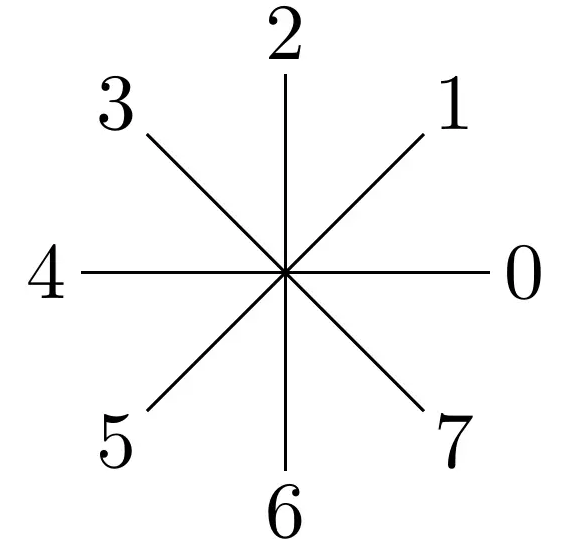
\includegraphics[width=0.2\textwidth]{direction.png}
    \caption{chemfig方向的定义}
    \label{fig:direction}
\end{figure}

举个乙烷的例子:

\begin{center}
  \chemfig{C(-[2]H)(-[4]H)(-[6]H)-C(-[2]H)(-[6]H)-H}
\end{center}

上述乙烷代码如下:
{\verb|\chemfig{C(-[2]H)(-[4]H)(-[6]H)-C(-[2]H)(-[6]H)-H}|}
代码中 (-[X]Y) 内的数字 X 就表示了内容 Y 的位置,其中中括号([ ])的位置通常紧跟在化学键(-、= 等)之后。例如2表示的就是向上的方向,4 表示向左,6 表示向右。

再画一个苯环:
\begin{center}
  \chemfig{*6(-=-=-=)}
\end{center}

%%%%%%%%%%%%%%%%%%%%%%%%%%%%%%%%%%%%%%%%%%%%%%%%%%%%%%

\section{图像布局}
\label{sec.figure}
\subsection{单图布局}

    这是一段随机插入的文本,用来填充模板布局,感受模板视觉效果。这是一段随机插入的文本,用来填充模板布局,感受模板视觉效果。这是一段随机插入的文本,用来填充模板布局,感受模板视觉效果。这是一段随机插入的文本,用来填充模板布局,感受模板视觉效果。这是一段随机插入的文本,用来填充模板布局,感受模板视觉效果。这是一段随机插入的文本,用来填充模板布局,感受模板视觉效果。
    
    这是一段随机插入的文本,用来填充模板布局,感受模板视觉效果。这是一段随机插入的文本,用来填充模板布局,感受模板视觉效果。这是一段随机插入的文本,用来填充模板布局,感受模板视觉效果。这是一段随机插入的文本,用来填充模板布局,感受模板视觉效果。这是一段随机插入的文本,用来填充模板布局,感受模板视觉效果。这是一段随机插入的文本,用来填充模板布局,感受模板视觉效果。

单图布局如图\ref{F.glut_single}所示。

\begin{figure}[hbt]
\centering
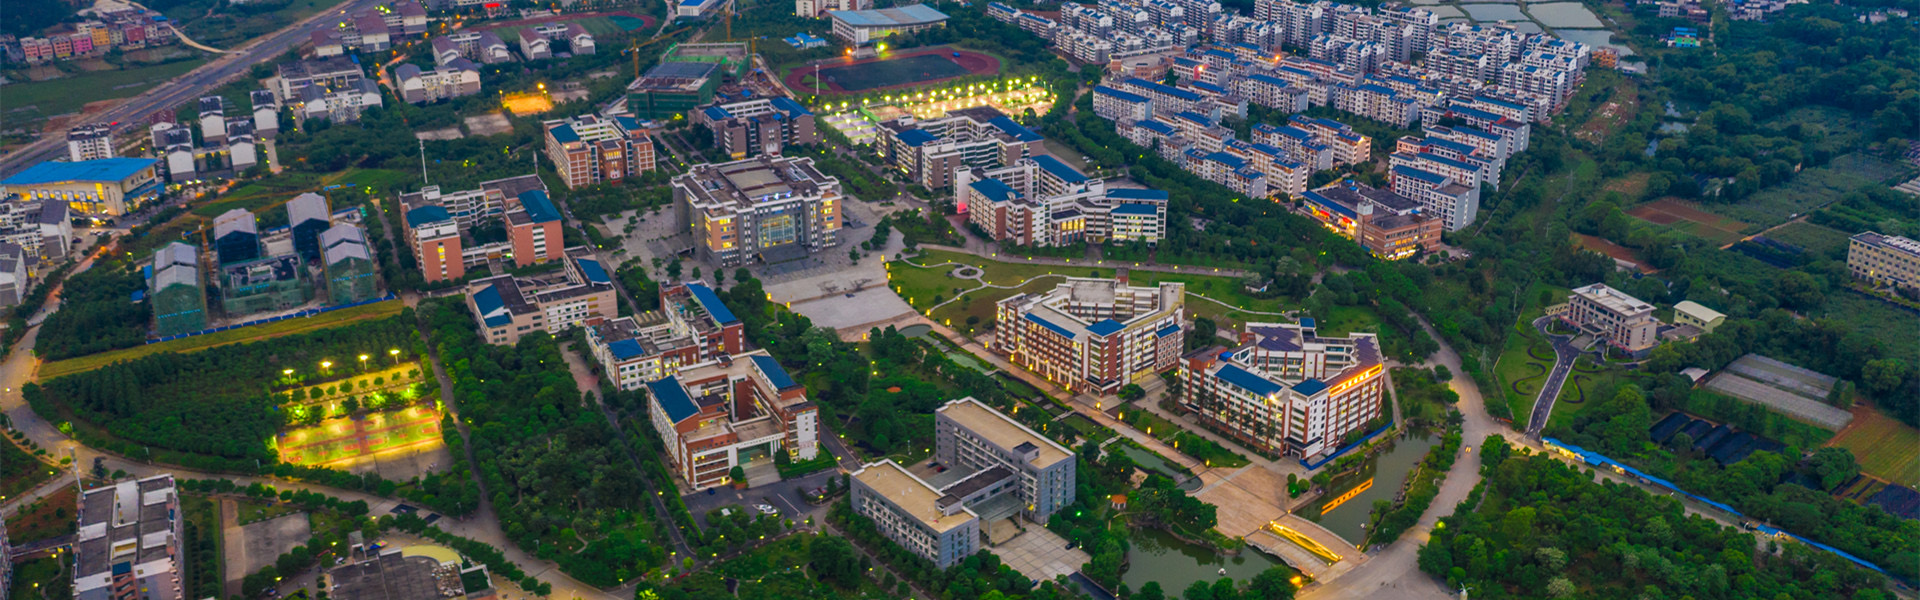
\includegraphics[width=1.0\textwidth]{banner.jpeg}
\caption{单图布局示例}
\label{F.glut_single}
\end{figure}

\subsection{横排布局}

横排布局如图\ref{F.glut_row}所示。

\begin{figure}[!htb]
    \centering
    \begin{subfigure}[t]{0.24\linewidth}
        \begin{minipage}[b]{1\linewidth}
        
\includegraphics[width=1\linewidth]{glut.png}
        \caption{第一张}
        \end{minipage}
    \end{subfigure}
    \begin{subfigure}[t]{0.24\linewidth}
        \begin{minipage}[b]{1\linewidth}
        
\includegraphics[width=1\linewidth]{glut.png}
        \caption{第二张}
        \end{minipage}
    \end{subfigure}
    \caption{横排布局示例}
    \label{F.glut_row}
\end{figure}

    这是一段随机插入的文本,用来填充模板布局,感受模板视觉效果。这是一段随机插入的文本,用来填充模板布局,感受模板视觉效果。这是一段随机插入的文本,用来填充模板布局,感受模板视觉效果。这是一段随机插入的文本,用来填充模板布局,感受模板视觉效果。这是一段随机插入的文本,用来填充模板布局,感受模板视觉效果。这是一段随机插入的文本,用来填充模板布局,感受模板视觉效果。
    
    这是一段随机插入的文本,用来填充模板布局,感受模板视觉效果。这是一段随机插入的文本,用来填充模板布局,感受模板视觉效果。这是一段随机插入的文本,用来填充模板布局,感受模板视觉效果。这是一段随机插入的文本,用来填充模板布局,感受模板视觉效果。这是一段随机插入的文本,用来填充模板布局,感受模板视觉效果。这是一段随机插入的文本,用来填充模板布局,感受模板视觉效果。

\subsection{竖排布局}
竖排布局如图\ref{F.glut_col}所示。

\begin{figure}[!htb]
    \centering
    \begin{subfigure}[t]{0.15\linewidth}
        \captionsetup{justification=centering} %ugly hacks
        \begin{minipage}[b]{1\linewidth}
        
\includegraphics[width=1\linewidth]{glut.png}
        \caption{第一张}
        \end{minipage}
    \end{subfigure}\\
    \begin{subfigure}[t]{0.15\linewidth}
        \captionsetup{justification=centering} %ugly hacks
        \begin{minipage}[b]{1\linewidth}
        
\includegraphics[width=1\linewidth]{glut.png}
        \caption{第二张}
        \end{minipage}
    \end{subfigure}
    \caption{竖排布局示例}
    \label{F.glut_col}
\end{figure}

    这是一段随机插入的文本,用来填充模板布局,感受模板视觉效果。这是一段随机插入的文本,用来填充模板布局,感受模板视觉效果。这是一段随机插入的文本,用来填充模板布局,感受模板视觉效果。这是一段随机插入的文本,用来填充模板布局,感受模板视觉效果。这是一段随机插入的文本,用来填充模板布局,感受模板视觉效果。这是一段随机插入的文本,用来填充模板布局,感受模板视觉效果。
    
    这是一段随机插入的文本,用来填充模板布局,感受模板视觉效果。这是一段随机插入的文本,用来填充模板布局,感受模板视觉效果。这是一段随机插入的文本,用来填充模板布局,感受模板视觉效果。这是一段随机插入的文本,用来填充模板布局,感受模板视觉效果。这是一段随机插入的文本,用来填充模板布局,感受模板视觉效果。这是一段随机插入的文本,用来填充模板布局,感受模板视觉效果。

\subsection{竖排多图横排布局}

\begin{figure}[!htb]
    \centering
    \begin{subfigure}[t]{0.13\linewidth}
        \captionsetup{justification=centering} 
        \begin{minipage}[b]{1\linewidth}
        
\includegraphics[width=1\linewidth]{glut.png} \vspace{-1ex} \vfill
        
\includegraphics[width=1\linewidth]{glut.png}
        \caption{第一张}
        \end{minipage}
    \end{subfigure}
    \begin{subfigure}[t]{0.13\linewidth}
        \captionsetup{justification=centering} 
        \begin{minipage}[b]{1\linewidth}
        
\includegraphics[width=1\linewidth]{glut.png} \vspace{-1ex} \vfill
        
\includegraphics[width=1\linewidth]{glut.png}
        \caption{第二张}
        \end{minipage}
    \end{subfigure}
    \caption{竖排多图横排布局}
    \label{F.glut_col_row}
\end{figure}

竖排多图横排布局如图\ref{F.glut_col_row}所示。注意看(a)、(b)编号与图关系。


\subsection{横排多图竖排布局}

    这是一段随机插入的文本,用来填充模板布局,感受模板视觉效果。这是一段随机插入的文本,用来填充模板布局,感受模板视觉效果。这是一段随机插入的文本,用来填充模板布局,感受模板视觉效果。这是一段随机插入的文本,用来填充模板布局,感受模板视觉效果。这是一段随机插入的文本,用来填充模板布局,感受模板视觉效果。这是一段随机插入的文本,用来填充模板布局,感受模板视觉效果。

\begin{figure}[!htb]
    \centering
    \begin{subfigure}[t]{0.3\linewidth}
        \captionsetup{justification=centering} 
        \begin{minipage}[b]{1\linewidth}
        
\includegraphics[width=0.45\linewidth]{glut.png}
        
\includegraphics[width=0.45\linewidth]{glut.png}
        \caption{}
        \end{minipage}
    \end{subfigure}\\
    \begin{subfigure}[t]{0.3\linewidth}
        \captionsetup{justification=centering} 
        \begin{minipage}[b]{1\linewidth}
        
\includegraphics[width=0.45\linewidth]{glut.png}
        
\includegraphics[width=0.45\linewidth]{glut.png}
        \caption{}
        \end{minipage}
    \end{subfigure}
    \caption{横排多图竖排布局}
    \label{F.glut_row_col}
\end{figure}

横排多图竖排布局如图\ref{F.glut_row_col}所示。注意看(a)、(b)编号与图关系。

\newpage
%%%%%%%%%%%%%%%%%%%%%%%%%%%%%%%%%%%%%%%%%%%%%%%%%%%%%%%

\section{表格插入示例}
表格如表\ref{T.example}所示,latex表格技巧很多,这里不再详细介绍。

\begin{table}[htb]
  \centering
  \caption{按照学术论文的一般规范,表格为三线表。}
  \label{T.example}
  \begin{tabular}{ccccc}
\toprule
A   &  B  &  C  & D  & E \\
\midrule
1 	& 一 & 壹 & one 	 & 啊\\
2 	& 二 & 贰 & two 	 & 哈\\
3 	& 三 & 叁 & three & 嗯\\
4 	& 四 & 肆 & four	 & 嘿\\
\bottomrule
\end{tabular}
\end{table}

\newpage

%%%%%%%%%%%%%%%%%%%%%%%%%%%%%%%%%%%%%%%%%%%%%%%%%%%%%%
\section{参考文献插入示例}

LaTeX\cite{lamport1994latex}插入参考文献最方便的方式是使用bibliography\cite{hu2020},大多数出版商的论文页面\cite{lamport1994latex}都会有导出bib格式参考文献的链接,把每个文献的bib放入``GLUTthesis.bib'',然后用bibkey即可插入参考文献。

\newpage
%%%%%%%%%%%%%%%%%%%%%%%%%%%%%%%%%%%%%%%%%%%%%%%%%%%%%%
\section{总结与展望}

XX的XX都存在XX,所以我们XX,本章总结XX。

\subsection{本文工作总结}
在总结和分析已有XX的理论基础上,本文对XX进行了XX,主要工作如下:

%手工编号
(1)图片插入布局,如第\ref{sec.figure}章所示。

(2)XXXXXXXXXX

(3)XXXXXXXXXX

(4)XXXXXXXXXX


\subsection{工作展望}
本课题针对XX,鉴于XXX,对XX进行了提高,但是XXX,所以有如下XX:

(1)目前XX虽然XX,但是XX仍然XX,所以XX仍然是一个值得XX的问题。

(2)随着XX,XX具有XX的问题,仍值得进一步XX。

(3)本课题在XX有了XX,但是XX的XX还存在XX,所以XX。

\newpage


%%%%%%%%%%%%%%%%%%%%%%%%%%%%%%%%%%%%%%%%%%%%%%%%%%
% 临时标签,用于编译时追踪正文末尾
%%%%%%%%%%%%%%%%%%%%%%%%%%%%%%%%%%%%%%%%%%%%%%%%%%

%%%%%%%%%%%%%%%%%%%%%%%%%%%%%%%%%%%%%%%%%%%%%%%%%%
% 后续内容,标题三号黑体居中,章节无编号
% --------------------------------------------%

% https://www.zhihu.com/question/29413517/answer/44358389 %
% 说明如下:
% secnumdepth 这个计数器是 LaTeX 标准文档类用来控制章节编号深度的。在 article 中,这个计数器的值默认是 3,对应的章节命令是 \subsubsection。也就是说,默认情况下,article 将会对 \subsubsection 及其之上的所有章节标题进行编号,也就是 \part, \section, \subsection, \subsubsection。LaTeX 标准文档类中,最大的标题是 \part。它在 book 和 report 类中的层级是「-1」,在 article 类中的层级是「0」。这里,我们在调用 \appendix 的时候将计数器设置为 -2,因此所有的章节命令都不会编号了。不过,一般还是会保留 \part 的编号的。所以在实际使用中,将它设置为 0 就可以了。

% 在修改过程中请注意不要破环命令的完整性

\renewcommand\appendix{\setcounter{secnumdepth}{-2}}
\appendix

% 主文件有代码去掉页眉章节编号的“.”,但这会因为bug导致无编号章节显示一个错误编号,所以这里在无编号章节之前再次重定义sectionmark。
%\renewcommand{\sectionmark}[1]{\markright{#1}}

% section 标题从这里往后改为三号居中
\titleformat{\section}{\centering \bfseries \zihao{3}}{\thesection}{1em}{}

% \section{参考文献} % bibliography会自动显示参考文献四个字
\addcontentsline{toc}{section}{参考文献} % 由于参考文献不是section,这句把参考文献加入目录
% \nocite{*} % 该命令用于显示全部参考文献,即使文中没引用
% cls文件中已经引入package,这里不需要调用 \bibliographystyle 了。
% \bibliographystyle{gbt7714-2005}
% \bibliography{thesis-references}
\printbibliography
\newpage

% 致谢应该在参考文献的后面,不编章号,而附录应该位于致谢后。
%!TEX root = ../GLUTthesis.tex
\section{致\quad 谢} % 无章节编号

% 公元二零二零年,岁次庚子,仲夏之月,吾之论文乃告杀青。辞穷理微,未敢称凌云之作,镂心鸟迹,得不效相如之叹?于是凭窗抱膝,寄情遐思。忆吾弱冠之龄入理工大学,意气方遒。尔来春秋有四,于今毕业,年齿已趋而立。户牅之外,万物滋荣,景致阙如昨日,堂室之内,吾已有苍颜白发矣。文凭两纸霜鬓两行,黄粱一枕功名一场,此皆寻常人生,乏善可陈。然吾身发受之父母,道德受之母校,学问受之师长,育教之恩,虽陨首结草不能报之万一。是以为情造文,铭而致谢。

大学四年即将结束,我也快要完成我的毕业论文,首先要感谢支持我完成论文的朋友。感谢我的指导老师王恒教授,给了我很大的发挥空间,在我对课题毫无头绪的时候指导我确定了具体的研究方向;感谢提供论文 \LaTeX 模板的胡光辉老师,他设计的论文模板让我不再被公式输入、排版等问题所困扰;感谢提供本文研究课题的巴灵丽同学,光孤子数值模拟问题来自她参加的夏令营的一个题目;感谢提供计算算力的裴俊杰同学,没有他的算力支持,我得不到有限差分的计算结果$\ldots\ldots$

其次要感谢生我养我的父母。我能来到这个世界这本身就是一件幸运的事,更何况是他们无微不至的关爱让我可以顺利健康地长大成人。小时候很淘气,给父母惹了很多麻烦;青春期比较叛逆,觉得父母老古董了,经常和他们对着干;长大了才发现,维持一个家庭,上有老,下有小是多么的不容易。父母正在老去,我要更加努力,为自己和社会创造更多价值,让他们不再操劳,能安度晚年。

最后要感谢陪伴我四年的桂林理工大学。感谢理学院的老师和同学,他们让我大学四年的学习生活不再孤单,经常给我提供帮助和建议以及挑战;感谢田径队的教练和队员,在大学因为共同的跑步爱好而聚在一起,互相鼓励、交流、提高,真的非常难得;感谢电子协会、数学建模协会和物理协会,让我大学四年的课余生活丰富多彩,社团活动给了我很多挑战,让我练出了非常多的技能$\ldots\ldots$即将离开母校,回想这四年,虽然有很多难熬的、烦心的事情,但是印象最深的还是那些奋斗过,快乐过的日子。
\newpage


%!TEX root = ../GLUTthesis.tex
\section{附录1} % 无章节编号
这里用来存放不应属于正文的内容、典型如代码、图纸、数学证明过程等内容。

物理常数表
\begin{table}[ht]
    \centering
 
    \begin{tabular}{lcll}
    \toprule 
          常数名称 & 符号 & 计算用值 & 单位 \\
    \midrule  

      真空中光速 & $c$ & $3.00\times 10^8$ & $\rm~ m\cdot s^{-1}$ \\
      
      万有引力常数 & $G$ & $6.67\times 10^{-11}$ & $\rm~ m^3\cdot s^{-2}$ \\
      
      阿伏伽德罗常数 & $N$ & $6.02\times 10^{23}$ & $\rm~ mol^{-1}$ \\

      玻尔兹曼常量 & $k$ & $1.38\times 10^{-23}$ & $\rm~ J\cdot K^{-1}$\\

      斯特藩-玻尔兹曼常数 & $\sigma$ & $5.67\times10^{-8}$ & $\rm~ W\cdot m^{-2}\cdot K^{-4}$\\ 
      
      理想气体摩尔体积 & $V_m$ & $22.4\times 10^{-3}$ & $\rm~ m^3\cdot mol^{-1}$ \\

      基本电荷 & $e$ & $1.60\times10^{-19}$ & $\rm~ C$\\

      电子静止质量 & $m_e$ & $9.11\times10^{-31}$ & $\rm~ kg$\\
      
      电子荷质比 & $e/m$ & $1.76\times10^{-11}$ & $\rm~ C\cdot kg^{-2}$\\

      质子静止质量 & $m_p$ & $1.67\times10^{-27}$ & $\rm~ kg$\\
      
      中字静止质量 & $m_n$ & $1.67\times10^{-27}$ & $\rm~ kg$\\
      
      $\alpha $粒子静止质量 &   & $6.645\times10^{-27}$ & $\rm~ kg$\\

      氢原子质量 & $m_\mathrm{H}$ & $1.67\times10^{-27}$ & $\rm~ kg$\\
      
      真空电导率 & $\varepsilon _0$ & $8.85\times10^{-12}$ & $\rm~ F\cdot m^{-2}$\\
      
      真空磁导率 & $\mu _0$ & $12.57\times10^{-7}$ & $\rm~ H\cdot m^{-1}$\\
      
      波尔半径 & $\alpha _0$ & $5.29\times10^{-11}$ & $\rm~ m$\\
      
      真空磁子 & $\mu _B$ & $9.27\times10^{-24}$ & $\rm~ J\cdot T^{-1}$\\
      
      普朗克常量 & $h$ & $6.63\times10^{-34}$ & $\rm~ J\cdot s$\\
    \bottomrule
    \end{tabular}
\end{table}

\newpage
%%%%%%%%%%%%%%%%%%%%%%%%%%%%%%%%%
\section{附录2} 


这是本设计所用的源程序代码:

\begin{lstlisting}[language={C}, caption={}]
/*程序:ex1_1.c */
/*功能:控制一个LED闪烁程序 */
#include <reg51.h>  /*包含头文件reg51.h,定义了51单片机的专用寄存器*/
sbit P1_0=P1^0;          	/*定义位名称*/
/*函数名:delay*/
/*函数功能:实现软件延时*/
/*形式参数:无符号整型变量i,控制空循环的循环次数*/
/*返回值:无
void delay(unsigned int i) 	/*延时函数*/
{
  unsigned int k;
	for(k=0;k<i;k++);
}
void main()                	/*主函数*/
{
  while(1){
     P1_0=0;				/*点亮LED*/
     delay(10000);			/*调用延时函数,实际参数为10000*/
     P1_0=1;				/*熄灭LED*/
     delay(10000);			/*调用延时函数,实际参数为10000*/
           }
 }

\end{lstlisting}


\end{document}
